\documentclass[a4paper,11pt]{article}

\usepackage[top=2cm, bottom=2cm, left=2cm, right=2cm]{geometry}

\usepackage{mathptmx}
\usepackage{epsf}           %\input{epsf}
\usepackage{amsfonts}
\usepackage{amstext}
\usepackage{amssymb}
\usepackage{url}
%\usepackage[dvips]{graphics}
\usepackage[dvips,pdftex]{graphicx}
\usepackage[dvips,all]{xy}
\usepackage{multicol}
\usepackage{natbib}
\setlength{\bibsep}{0.0pt}

\usepackage{hyperref}

%\newlength{\extraplusheight}
%\newlength{\extrapluswidth}
%\setlength{\extraplusheight}{4.7cm}
%\setlength{\extrapluswidth}{4.7cm}
%\addtolength{\textwidth}{\extrapluswidth}
%\addtolength{\textheight}{\extraplusheight}
%\addtolength{\oddsidemargin}{-.5\extrapluswidth}
%\addtolength{\evensidemargin}{-.5\extrapluswidth}
%\addtolength{\topmargin}{-0.5\extraplusheight}
\setlength{\parindent}{0 pt}
\setlength{\parskip}{1ex}

\newcommand{\eg}{{e.g.}\ }

\newcommand{\Int}[1]{[\![ #1 ]\!]}
\newcommand{\malign}[1]{\begin{array}[t]{@{}l@{\;}l@{}l@{}} #1 \end{array}}
\newcommand{\logrel}[2]{\Delta_{#1,#2}}
\newsavebox{\fminibox}
\newenvironment{fminipage}
 {\begin{lrbox}{\fminibox}\begin{minipage}{8cm}\vspace*{-2ex}}
 {\\[-2ex]\vspace*{-2ex}\end{minipage}\end{lrbox}\noindent\centerline{\fbox{\usebox{\fminibox}}}\vspace{0.5ex}}   

%\setlength{\parindent}{0.15in}
%\setlength{\parskip}{0.3ex}

% Discourage unnecessary hyphenation.
\sloppy\hyphenpenalty 4000

\newcommand{\ra}{\rightarrow}
\newcommand{\A}{\mathcal{A}}
\newcommand{\E}{\mathcal{E}}
\newcommand{\C}{\mathcal{C}}
\newcommand{\B}{\mathcal{B}}
\newcommand{\Set}{\mbox{{\sf Set}}}
\newcommand{\Nat}{\mathit{Nat}}
\newcommand{\Alge}[1]{\mathit{Alg}_{#1}}
\newcommand{\hash}{\#}

\begin{document}

\thispagestyle{plain}
\begin{center}
  {\Large {\bf Homotopy Type Theory: Programming and Verification}}\\[1ex] 

\vspace*{-0.1in}

%  {\Large \bf Case for Support}\\[1ex]
  \rule{140mm}{.5mm}\\[2ex]
\end{center}

\noindent
{\bf \Large Part 1A: Previous Research \& Track Record}

\textbf{Professor Neil Ghani.} Neil Ghani earned his PhD in Computer
Science in 1995 from the University of Edinburgh, where he worked on
categorical models of rewriting.  After becoming a Lecturer at
Leicester and then a Reader at Nottingham he was appointed to a
professorship at the University of Strathclyde where he founded the
Mathematically Structured Programming (MSP) group. His research has
focussed on a number of topics directly related to the subject of the
current proposal, \eg (1) his work on data types (containers, quotient
containers, indexed containers and induction recursion) is directly
related to our plans in WP3 to develop the theory of higher inductive
types; (2) his work on logical relations is directly related to our
plans in WP1 and WP2 to develop the model theory for HoTT as well as
the syntactic presentation of this model theory as a type theory; (3)
his work on the semantics of effects is directly related to the
application of HoTT to effects as planned in WP4; and (4) his work on
Units of Measure (via an IAA grant held in collaboration with
Microsoft) directly relates to WP8 which applies HoTT to computing
with algebraic structures such as within Units of Measure. Indeed,
results obtained during his previous EPSRC grants on Containers,
Induction Recursion and Logical Relations will feed into this
proposal.  More generally, Neil Ghani is a world expert on the use of
semantic structures to drive the development of type theory and
programming languages, exactly the methodology to be followed in this
proposal.

Professor Ghani serves as a member of the EPSRC College charged with
assessing the quality of grant applications. He is also a grant
assessor for the Carnegie Trust.  He was the director of the Midlands
Graduate School in the Foundations of Computer Science, is a SICSA
theme leader in Complex Systems Engineering, and was on the Steering
Committee for the British Colloquium on Theoretical Computer Science.
He has served on numerous programme committees and been the external
examiner for a number of PhD students. He is also Deputy Head of
Department and Head of Research in his home Department. He has
successfully supervised five PhD students and four RAs and has
experience in the successful management of large grants. He organises
the Scot Cats seminar series, and plans to host a meeting in the UK on
Homotopy Type Theory in November 2014, both of which puts him in touch
with other experts in the area.

For further information, see~\url{http://www.cis.strath.ac.uk/~ng}

\textbf{Dr Conor McBride.} Conor McBride received his PhD from the
University of Edinburgh in 1999 for his work on dependently typed
programming. After this, he worked as an RA at the Universities of
Durham and Nottingham before becoming a lecturer at the University of
Strathclyde in 2008. His work on the foundations and implementations
of non-dependently and dependently typed programming as become very
influential, both via his own programming language Epigram and via his
work with the Agda, Coq and Haskell teams. He is now widely regarded
as a leader of his field as illustrated by his widely cited papers,
journals, and invitations to keynote addresses at conferences
etc. Apart from the evident importance of this expertise for WP6 and
WP7, Dr McBride's work on OTT, on containers and on effects feed into
WPs 3 and 4. Since becoming a lecturer, Dr McBride has had two grants
funded by EPSRC and - importantly - one by Microsoft. Not only are all
of these grants of direct relevance to this project, but these grants
show both his experience of working in large distributed grants and
that our plans for generating industrial impact through collaborations
with Microsoft are built on solid and successful pre-existing
foundations. Dr McBride has also supervised two PhD students and
currently supervises a further two students. He also leads the MSP
group.

For further information,
see~\url{https://personal.cis.strath.ac.uk/conor.mcbride/}

\textbf{Host Institution: The University of Strathclyde.} The MSP
group at the University of Strathclyde is an ideal venue for
conducting this research. Led by Conor McBride, the group includes
Prof Ghani, Dr Clemens Kupke, Dr Ross Duncan as well as two research
associates and seven PhD students. The MSP groups vision is to use
mathematics to understand the nature of computation, and to turn that
understanding into the next generation of programming languages. That
is exactly the methodology used within this proposal and hence this
proposal will both benefit from, and benefit, the MSP group.
Finally, central Scotland is home to vibrant theoretical computer
science and functional programming research communities, and the
University of Strathclyde is an active participant in the Scottish
Informatics and Computer Science Alliance (SICSA). The MSP group also
is active in other Scottish meetings, such as ScotCats and SPLS.

\textbf{Dr Thorsten Altenkirch.}  Thorsten Altenkirch received his PhD in
Computer Science from the University of Edinburgh in 1993. Since 2006
he is Reader at the University of Nottingham,
where he founded the Functional Programming Laboratory with Graham
Hutton in 2008. Altenkirch is well known for his work on type theory
and applications of category theory in computer science, and has
published over 50 research papers which are frequently cited (h-index~$\geq 26$). During his
work at Nottingham he attracted \pounds 1M in research funding,
comprising~\pounds650,903 as PI in 4 EPSRC grants, \pounds241,075 as
CoI in 2 EPSRC grants, \pounds159,038 in 1 fellowship and 1
studentship. Especially relevant for the current project is
Observational Equality For Dependently Typed Programming
(EP/C512022/1), Theory And Applications of Induction Recursion
(EP/G03298X/1), Reusability and Dependent Types
(EP/G034109/1). Altenkirch and Ghani have already collaborated
successfully on three research grants. More generally, 
Altenkirch is one of the leading researchers on HoTT
This is witnessed by his fellowship at the Institute of Advanced Study
in Princeton in occasion of the special year on the subject in 2013. There, he contributed to the standard reference on the
subject~\cite{hott-book}.  He has given invited lectures on the
subject (at HDACT in Lubljana in 2012, at the Curien-fest in Venice in
2013, at MSC in Lyon and at the Institut Henri Poincar\'e in Paris in
2014). He has already published several papers on HoTT
\cite{altenkirch:extSetoids,alti:ott-conf,alti:csl12,alti:tlca13-hedberg}.

For further information, see~\url{http://www.cs.nott.ac.uk/~txa}

\textbf{Host institution: The University of Nottingham.}  The
University of Nottingham is one of the leading Universities in the UK
and its School of Computer Science was ranked 8th in the last Research
Assessment Exercise. The Functional Programming Lab (FP Lab) within the School
is one of its four major research groups, with an international
reputation for its work on formally-based approaches to software
construction and verification.  The FP Lab currently comprises 4
academic staff: Professor Graham Hutton, Dr Thorsten Altenkirch, Dr
Venanzio Capretta, and Dr Henrik Nilsson and nine PhD students.  To
date, the group has received~\pounds1.5M of EPSRC funding over 14
projects, and has 12 completed PhD students.  The FP Lab provides a highly stimulating research environment,
holds weekly research seminars and is also a leading participant in the MGS - a
collaborative venture with Leicester and Birmingham offering training
to PhD students.
\noindent

\textbf{Dr Nicola Gambino.} Nicola Gambino received his PhD in
Computer Science from the University of Manchester in 2002. After
carrying out postdoctoral research, he became an Assistant Professor
in Mathematical Logic at the University of Palermo in 2008. Since
September 2012, he is an Associate Professor in Pure Mathematics at
the University of Leeds. Nicola Gambino is one of the leading
researchers on HoTT: 
i) his work on constructive mathematics and
homotopical algebra~\cite{GambinoN:homl2c,GambinoN:weilsh} feeds into
semantic models of HoTT in WP1; ii) he obtained~\cite{gambinoGarner:ITwfs} one of the first results
relating type theory and homotopy theory feeds into WP2 
iii) his research on polynomial data;
types~\cite{gambinoHyland:welfoundedTrees,GambinoN:polfpm}, and
especially his recent work on inductive types in Homotopy Type
Theory~\cite{awodeyGamSoja:indTypesInHTT} feeds into WP3 on higher
inductive types; iv) his experience in proof theory and formalization
of proofs in Coq will be beneficial for WP5, where we machine check
our results.

Nicola Gambino has a consistent record of
publications in leading journals and of invited lectures at
international conferences, {e.g.}~at the 2010 Logic Colloquium in Paris
and at the forthcoming joint 2014 RTA-TLCA conference in Vienna. He
held visiting positions at leading research centres, including the Institut Mittag-Leffler (Stockholm), the
Fields Institute (Toronto) and the Institute of Advanced Study
(Princeton), where he worked with Vladimir Voevodsky (the inventor of
the Univalence Axiom).  He is currently an invited researcher to the
Institut Henri Poincar\'e (Paris) for the special trimester on
Semantics of Proofs and Certified Mathematics.  He is an editor of the
journal Mathematical Structures in Computer Science.
He supervises
an RA (funded by the US Air Force Office for Scientific
Research) working on the foundations of HoTT. 

For further information,  see~\url{http://www.maths.leeds.ac.uk/~pmtng}.

\textbf{Host Institution: The University of Leeds.} The University of
Leeds is one of the leading universities in the UK and provides
excellent facilities for research. The School of Mathematics hosts the
Mathematical Logic group, which includes seven members of staff, four
research fellows and nineteen research students. The group has a
vibrant research profile; in particular, it frequently organises
international conferences and runs several regular activities,
including a weekly Mathematical Logic Colloquium as well as specialist
seminar series in model theory, proof theory and computability
theory. The Mathematical Logic group has been consistently funded by
EPSRC and international agencies and is already active on Homotopy
Type Theory. In particular, we intend to collaborate closely with
Professor Michael Rathjen who is currently PI
on a 3-year EPSRC grant on proof-theoretical aspects of HoTT. 

\newpage

\noindent
{\bf \Large Part 2: The Proposed Research and Its Context}

\vspace*{-0.23in}

\begin{center}
\rule{170mm}{.5mm}
\end{center}

\vspace*{-0.4in}

\section{Introduction}\label{sec:intro}

\vspace*{-0.1in}

{\bf Formal Verification.} The cost of software failure is truly
staggering\footnote{see the section on National
  Importance.}. Traditional methods of software verification based
upon testing only generate partial guarantees of correctness. Stronger
guarantees of software correctness are given by mathematical proofs
but the complexity of modern software means that hand written
mathematical proofs are untrustworthy. As a result, the only way to
ensure truly secure and reliable software is the gold standard of
formally verified software, which offers machine-checked mathematical
proofs of software correctness. Several decades of pioneering work in
the UK and elsewhere has culminated in systems 
such as Agda, Coq, Epigram, Idris, NuPRL, Twelf, and
the Trellys project which are now having significant impact,
\eg Coq has won both the 2013 ACM Software award and the 2013 SIGPLAN
Programming Languages Software award. The advanced type-theoretic
technology of these systems is also raided by more mainstream languages
with significant industrial deployment such as Haskell, OCaml, Scala
and C\#.

%SWIFT
%Other prizes for other systems
%Economy of Trust

{\bf The Project.} Despite their success, such systems have several
fundamental limitations, \eg when programming with quotients,
supporting abstraction (that is, invariance under different
representations of the same structure) and extensional reasoning
(proving that programs which behave the same are the same).  {\em
  Homotopy Type Theory} (HoTT) is widely regarded as a fundamental
innovation with great potential to address these and other problems.
To realise this potential, we propose a synthesis of
theoretical, applied and impact-focussed research.


%Delivering this potential requires i) further development of the
%foundations of HoTT; ii) programming language and verification tools
%based on these foundations; and iii) applications demonstrating their
%effectiveness to the broader community.  Therefore we i
%The key concept in HoTT is to introduce a very liberal
%equality which identifies structures that are replacable.

%Its core is Voevodsky's {\em Univalence Axiom} asserting
%that all provable equalities can be internalised as paths or, more
%conceptually, that computation is invariant under change of
%representation of the entities we compute with.


$\;\;\; \;\;\;$ {\em Theoretical Foundations.} Almost all of our understanding
  of HoTT exists within a classical framework and hence cannot be used
  to develop programming language and verification tools. Nevertheless, the recent
  work by Coquand et.al.~\cite{BezemM:cubsmt} strongly suggests a constructive presentation of HoTT
  is possible. We will develop both specific constructive models
  and a general constructive model theory of HoTT, and then complement
  these models with type theoretic presentations of them.

$\;\;\;\;\;\;$ {\em Programming Language and Verification Tools.} The key
  deliverable of the second strand of our research will be a
  programming language which simultaneously acts as a verification
  environment based upon HoTT. This is likely to become a major
  step forward in programming languages design and influence
  the development of all current and future systems in this area.

$\;\;\;\;\;\;$ {\em Generating Impact.} Developing new and fundamentally
  better ways to construct formally verified software is not just an
  end in itself, but is also a key prerequisite for engaging others to
  do the same.  To help ensure this, we will produce a number of case studies so
  users can learn from, and experiment with, our results. At the same time, their
  practical experiences with it will feed back into our research.

  {\bf Calibre, Ambition, and Adventure.} The potential of HoTT to
  solve one of the deepest problems in programming languages and
  verification - namely the efficient computational treatment of
  equality/representational invariance - demonstrates our ambition to
  fundamentally transform the construction and validation of software.
  The proposal's calibre is demonstrated by the depth and range
  of the state-of-the-art ideas we will deploy in our
  research. Finally, the proposal's adventure
  is demonstrated by its scope, ranging from fundamental research
  (WP1,2,3) to programming languages and verification (WP5,6,7) 
  to impact generation via case studies (WP4,8).

\vspace*{-0.1in} 

% %txa: added heartbleed.
% %{\bf Cost of Software Failure:} The cost of software failure is truly
% %staggering. Well known individual cases include the Mars Climate
% %Orbiter failure ($\pounds 80$ million), Ariane Rocket disaster
% %($\pounds 350$ 
% %million), Pentium Chip Division failure ($\pounds 300$ million), most recently
% %the heartbleed bug (upto $\pounds 250$K per server) and there are
% %many, many more examples. Even worse, other software failures such as
% %one in the Patriot Missile System and another in the Therac-25 radiation system
% %have costs lives. More generally, a 2008 study by the US
% %government estimated that faulty software costs the US economy
% %$\pounds 40$ billion annually.  As a result, the human and economic
% %importance of ensuring programs run without error is hard to
% %over-estimate.
 

% %The worldwide software market is estimated at
% %\pounds 250 billion pounds every year and this figure will grow
% %significantly in real terms as software becomes ever more ubiquitous
% %in our lives and economy. Although the requirements for software vary
% %enormously, a problem common to all software is to ensure programs run
% %without error. Restarting a phone is a simple, if inconvenient task;
% %restarting an aeroplane in mid-flight is not an option! Numerous
% %examples of expensive software errors about from the Mars Rover to be
% %recent Heartbleed Bug exposing a serious vulnerability in the popular
% %OpenSSL cryptographic software library.  In a nutshell, the cost of software bugs is almost
% %unbelievably staggering.

% {\bf Formal Verification.} The cost of software failure is truly
% staggering\footnote{see the section on National
%   Importance.}. Traditional methods of software verification based
% upon testing only generate partial guarantees of correctness. Stronger
% guarantees of software correctness are given by mathematical proofs
% but the complexity of modern software means that hand written
% mathematical proofs are untrustworthy. As a result, the only way to
% ensure truly secure and reliable software is the gold standard of
% formally verified software, which offers machine-checked mathematical
% proofs of software correctness. Several decades of pioneering work in
% the UK and elsewhere have culminated in prototype languages and tools
% such as Agda, Epigram, Idris and Coq and in the US NuPRL, Twelf, and
% the Trellys project. These systems are beginning to make their mark,
% \eg Coq has just won both the ACM Software award and the SIGPLAN
% Programming Languages Software award.
% %~\cite{}.  -not needed, txa
% The advanced
% type-theoretic technology of these systems is raided by more
% mainstream languages with significant industrial deployment such as
% Haskell, OCaml, Scala and C\#.

% {\bf The Project.} Despite these successes, such systems have a number
% of short comings in crucial areas, \eg when programming with quotient
% types, supporting abstraction (that is, invariance under different
% representations of the same structure) and extensional reasoning
% (proving that programs which behave the same are the same).  {\em
%   Homotopy Type Theory} (HoTT) is widely regarded as a fundamental
% innovation with great potential to address these and other problems.
% Delivering this potential requires i) further
% development of the foundations of HoTT; ii)
% a programming language and verification environment based on
% these foundations; and iii) applications demonstrating the effectiveness
% of this environment to the broader software development community.
% Therefore we intend to pursue a three-pronged
% research programme based upon a synthesis of theoretical, applied and
% impact-focussed research.

% %The key concept in HoTT is to introduce a very liberal
% %equality which identifies structures that are replacable.

% %Its core is Voevodsky's {\em Univalence Axiom} asserting
% %that all provable equalities can be internalised as paths or, more
% %conceptually, that computation is invariant under change of
% %representation of the entities we compute with. 



% \begin{itemize}
% \item {\bf Theoretical Foundations.} Almost all of our understanding
%   of HoTT exists within a classical framework and hence cannot be used
%   to develop programming language and verification tools. Nevertheless, the recent
%   work by Coquand et al. strongly suggests a constructive presentation of HoTT
%   is possible. We will develop both specific constructive models
%   and a general constructive model theory of HoTT, and then complement
%   these models with type theoretic presentations of them.
% \item {\bf Programming Languages and Verification:} The key
%   deliverable of the second strand of our research will be a
%   programming language which simultaneously acts as a verification
%   environment based upon HoTT. This is likely to become a major
%   step forward in programming languages design and influence
%   the development of all current and future systems in this area.
% \item {\bf Generating Impact:} Developing new and fundamentally
%   better ways to construct formally verified software is not just an
%   end in itself, but is also a key prerequisite for engaging others do
%   do so.  To help ensure uptake of our research by the wider
%   community, we will produce a number of case studies which will allow
%   users to experiment with our results; at the same time, their
%   practical experiences with it will feed back into our research.
% \end{itemize}

% {\bf Calibre and Ambition.} The foundational nature of HoTT, the
% consequent potential for solving key open problems in programming
% languages and formal verification research, and the resulting
% potential applications to software correctness attest to the quality
% and calibre of this project. Our ambition is demonstrated by the
% breadth of our central belief that HoTT is not just a mathematical
% foundation for type theory, but can also be turned into a programming
% language and verification environment which - in its treatment of
% quotients, representational invariance and equality - will become the
% benchmark standard which current and future systems will seek to
% emulate.

\vspace*{-0.1in} 
\section{Scientific and Technological Background.}
\vspace*{-0.1in} 

{\bf Programming Languages.} Abstraction is essential in programming
as identifying common structure ensures code is clear,
clean and concise. This has lead to the development of high level
programming languages with expressive type systems capable of closing
the {\em semantic gap} between what programmers know about
computational entities and what their types can express about them.
The current state of the art are the {\em dependently typed
  programming languages} mentioned above where
the type of a program can express a
continuum of precision - from basic assertions up to a complete
specification - about the program’s behaviour. This proposal seeks to
develop the first of a new breed of 
such programming languages which advance the state of the art by offering a
powerful yet computationally tractable equality, and thereby bring to
reality the goal of programming up to invariance of representation.

%Coq award
%transform
%ahead of the curve

{\bf Program Verification.} While the advantages of the certainty
afforded by mathematical proof has been recognised for centuries, it
has also been recognised that this certainty is undermined by the
capacity for humans to make mistakes in their proofs. The advent of
computers raised the possibility once more of achieving in practice
the promise of mathematical certainty. This potential is now coming to
fruition, \eg systems such as Coq have been able to formally verify
both large mathematical theorems such as the 4-Colour problem, and
large software systems such as the CompCert C-compiler. However, these
systems are not {\em extensional} as objects which are behaviourally
indistinguishable cannot be proven the same and this fundamental problem
significantly weakens the power of the verification system. In contrast, our
research will produce a formal verification system where objects
with the same behaviour can indeed be proved equal.


{\bf Type Theory.} Underlying formal verification systems and
programming languages is the subject of type theory which grew out of
Russell's attempts to deal with paradoxes in naive set theory. A major
step forward was the Curry-Howard correspondence which observed that
programs and proofs are actually the same thing, \eg proofs are just
particular forms of programs. As a result, by developing sophisticated
type theories, we advance both the fields of programming languages and
program verification. Another major advance was Martin-L\"of's realisation
that type theory needed to be extended to cover equality within the
system. %This produced a sophisticated theory because not only could
%one talk about proofs of the equality of terms, but also proofs that
%such proofs were in fact the same.
To do this, he introduced the intensional equality type in
Martin-L\"of Type Theory (MLTT).  However, it soon became apparent
that this equality type was too weak, \eg functions that are pointwise
equal cannot be proven equal. Martin-L\"of then
introduced extensional MLTT which produced a strong equality but at
the price of losing decidability of type checking. Fundamentally, the
problem of a strong but decidable equality has remained
unresolved for 40 years - HoTT is exciting precisely because
it seems to offer a genuine advance on this most fundamental of problems. 


{\bf Observational Type Theory} (OTT) is a step towards a decidable
type theory with a strong equality, proposed by Altenkirch and
McBride~\cite{alti:ott-conf}. Unlike the equality type of Martin-L\"of
which defined equality uniformly for all types, OTT defines equality
by induction on the structure of types (and is thus extensional) while
its definitional equality remains decidable. However, the {\em
  equality of types} themselves is rigidly structural which means it
is not strong enough to convert proofs about one type to proofs about
an equivalent type. As HoTT can be seen as a higher dimensional
extension of OTT, our experience in OTT will invaluable in offering key
insights and techniques for its development.

{\bf Logical Relations.} Another important background technology is
logical relations which again uses induction on type structure to
define not equlities, but rather relations, over all types. Logical
relations have already been used~\cite{LicataHarper} to study a
truncated form of HoTT. Moreover, what is
particularly interesting is that Coquand's cubical sets
model~\cite{BezemM:cubsmt} is closely related to logical relations
because cubical sets arise naturally when one extends logical
relations to higher dimensions via the pattern of set, relation,
relation between relations etc. Ghani's research into logical relations is
currently being funded by EPSRC at Strathclyde and we will use our
results to see if higher dimensional variants of the standard
presentations of logical relations (eg Kripke or mixed arity logical
relations) lead to better behaved refinements of the cubical sets
model. 



%power of methods
%absolutely vital
%very clear evidence

% invariance of representation = iso == equal
%vs
% strength of propositional equality (= identity type)
% strength of definitional equality beta

% hott or univalence
% hott = tt + univalence + hits
% univalance + hdtt/hdct
% hott = int param + kan filllers + hits
% what does univalence mean

{\bf Homotopy Type Theory.} HoTT is a revolutionary new analysis of
equality based on intuitions from homotopy theory. Types are
\emph{spaces}; terms are \emph{elements} within a space; the equality
type is the space of \emph{paths} in a space. The core of HoTT is the
new Axiom of Univalence, introduced by Fields medalist Vladimir
Voevodsky, asserting (roughly) that isomorphic types are
equal. Crucially, equality proofs carry the data necessary to program
and reason up to invariance of representation. HoTT subsumes function
extensionality but also transcends what we could previously express,
e.g.\ \emph{higher} inductive types (HITs) include the usual tree
structures, but also quotients \cite{alti:mpc04} and geometric objects such as the
torus, where the hole stops us deforming some paths into others. Such
paths contain non-trivial structural information, necessitating a
proof-relevant equality. The same phenomenon occurs in computer
science, e.g. lists are an inductive type; braids are lists with extra
paths identifying lists up to twisting of any element past its
neighbours, and bags are braids with paths-between-paths identifying
braidings which yield the same permutation.

The model of HoTT based on \emph{cubical sets} currently being developed~\cite{BezemM:cubsmt} interprets closed expressions
as canonical denotations, which leads to basic feasibility of computing
with the Univalence Axiom. However, much work lies ahead: we need to give
closed expressions normal forms \emph{within} HoTT, and to recover
definitional equalities lost by the cubical interpretation (such as the one in the
computation rule for identity types). Further, other models might
offer better computational foundations for HoTT, so practical progress
towards programming languages and verification tools based on HoTT
needs a broader model theory.



%txa: replacing
% One of the key features of Coquand's model is that
% the equality relation is defined recursively over the structure of
% types using an internalised form of parametricity. 




% Nevertheless, Coquand's and Huber's
%work shows that producing programming languages and proof assistants
%based upon HoTT is feasible in principle and we plan to
%collaborate closely with them.


%Earleir motivation for OTT
%Grant numbers below

%Mention somewhere the prizes that Coq has been recently been awarded, as proof that this is cutting-edge technology

%Mention somewhere that HoTT is having an impact on the design of (new versions of) Coq: there is ongoing work on implementing mechanisms for higher inductive types (Barras). Also: Bauer is working on new proof assistant based on ideas of Voevodsky.

%Mention somewhere also the importance of type theory, Coq, Agda for
%computer-assisted formalization of mathematical proofs 

%Why us and not the United States of Awodey. Strong definitional
%equlity. 

\section{Methodology and Research Programme}



Our general methodology to the development of HoTT-based software
construction and verification will be to harness ideas from a number
of different sources: i) the evolving state of the art, e.g. the HoTT
book and the cubical sets model  as well as
the ongoing dialogue with our collaborators; ii) our work on OTT which
is a proof-irrelevant prototype of what we seek; iii) our work on the
implementation of dependently typed programming languages (Epigram and
$\Pi\Sigma$ \cite{alti:pisigma-new,alti:checking}); iv) our work on datatypes (containers, indexed
containers, induction-induction and induction-recursion) 
\cite{alti:fossacs03,alti:tlca03,alti:icalp04,alti:jpartial,alti:mpc04,alti:cont-tcs,alti:regular,alti:cats07,alti:jcats07,alti:lics09,
alti:catind2}
 ; v) our work
on parametricity; and vi) our work on constructing internal models of
type theory. These multiple sources will ensure that we neither
slavishly follow the hype that inevitably surrounds significant
innovation, nor are unaware of current and future advances in HoTT. We
have divided the project into the following work packages with WP1
hosted in Leeds, WP2-4 in Nottingham and WP5-8 in Strathclyde. Of course
the reality is that we will continue our established practice of
working closely together.

%Argue in justification for resources
%Explain compute below 



{\bf WP1: Semantic Foundations of HoTT.}  We seek semantic insights
for HoTT akin to those provided by Cartesian closed categories for
the simply typed $\lambda$-calculus.  A constructive model theory for
HoTT is essential because: (1) a general model theory 
guides the design of different presentations and implementations of
HoTT; (2) models of HoTT provide algebraic techniques to reason
about the correctness of implementations which complement syntactic
techniques, and in particular (3) specific implementations of HoTT can
be proven sound by giving a specific models of them.  These models
need to be constructive so that programs, even those using the
Univalence axiom, will compute ({i.e.} reduce to a normal form). While
the standard model of HoTT based upon simplicial sets is not
constructive, the cubical sets model currently being developed~\cite{BezemM:cubsmt} is constructive and raises the question of understanding it
within a general model theory.

 We will attack this problem from the following directions: (1) we
 will analyse existing models ({e.g.} groupoids~\cite{HofmannM:groitt}, strict
 $\omega$-groupoids~\cite{WarrenM:strgit}, simplicial sets~\cite{KapulkinC:simmuv}, cubical sets~\cite{BezemM:cubsmt}) and isolate
 exactly how they ensure constructivity or where they fail to do
 so. In the latter case, we will investigate whether it is possible to
 constructivize them; (2) on the basis of our experience with (1), we
 will develop a model theory for HoTT by isolating the essential
 features of these models (especially those amenable of a constructive treatment)
 and  adapting known methods to construct Quillen model structures
 to the setting of HoTT ({c.f.}~\cite{ShulmanM:uniidh}, which however does not cover the cubical sets model).

For (2), our starting point will be recent advances in axiomatizing the
notion of a model of type theory in a simple way ({e.g..}~\cite{AwodeyS:natmtt}). On that basis, we will require the existence of additional
structure, corresponding to the axioms of HoTT under consideration. In
terms of risk, (1) is certainly achievable since it involves only the
analysis of existing concrete models, while (2) is a more ambitious
goal. Nevertheless, our expertise on semantics of type
theories~\cite{neil2014relParamDep}, homotopical
algebra~\cite{GambinoN:homl2c,GambinoN:weilsh} and
$\omega$-groupoids~\cite{alti:csl12} makes even this ambitious goal
feasible. Deliverables from WP1 will be a broad class of models of
HoTT which considerably deepen our understanding and map out the
design space of its syntactic presentations.

% {\bf WP1: Semantic Foundations of HoTT:}  We
% seek semantic insights into HoTT akin to those provided by Cartesian
% closed categories for the simply typed
% $\lambda$-calculus.  A constructive model theory for HoTT is essential because: i)
% specific implementations of HoTT can be proven sound by giving a specific
% models of them; ii) 
% %since we don't know a priori what the best implementation
% %of HoTT will be, 
% a general model theory of HoTT will implicitly predict, and thereby
% guide, the design space of different presentations and implementations
% of HoTT; and iii) models of HoTT will provide algebraic techniques to
% reason about the correctness of implementations which complement
% syntactic techniques. These models need to be constructive so that
% programs, even those using Univalence, will compute. While the
% standard model of HoTT based upon simplicial sets is not constructive,
% Coquand et al.'s recent cubical set model is constructive and 
% has thus opened the door to a more general model theory.

% %Joyal
% %Back ground : Qullien model structures

% We will attack this problem from the following directions: i) we will
% analyse existing models (cubical sets, groupoids, strict
% $\omega$-groupoids, simplicial sets, globular sets) to isolate exactly
% how they ensure constructivity, or (where they fail to do so) how to 
% constructivize them; and ii) informed by i),
% we will develop a model theory for HoTT by both adapting known methods to
% define Quillen model structures (such as the small object argument)
% to the constructive setting and by showing how one can build  new
% constructive model structures from old (\eg by
% slicing). A promising starting point for a constructive
% version of the small object argument comes from Garner's work, where
% it is related to the construction of free monads. In terms of risk,
% i) is certainly achievable since it involves only the analysis of
% existing concrete models, while ii) is a more ambitious
% goal. Nevertheless, our expertise on semantic models of parametricity \cite{neil2014relParamDep}, model
% categories (Gambino) and $\omega$-groupoids \cite{alti:csl12} makes even this
% ambitious goal feasible. Deliverables from WP1 will be a broad class
% of models of HoTT which considerably deepen our
% understanding and map out the design space of its 
% syntactic presentations.

% back ground work: NOMINAL SETS,

%LARGE BODY OF
%WORK ON SIMPLICIAL SETS AND MODEL CATEGORIES. MANY MODELS =>
%UNIVERSALLY VALID PRINCIPLES.
% Design space of the HoTT family earlier om

%Background: current presentation (HoTT presentation and Thierry's)
%dont have canonicity.

{\bf WP2: Univalent Type Theory.} Building on WP1, we need syntactic
presentations of our models of HoTT in the form of type theories. The
challenge is to present the essential data of the model as built from
a {\em finite} collection of type and term constructors - this is
particularly difficult given the {\em arbitrary} higher dimensional
structure of HoTT. One also must prove essential properties such as strong normalisation, decidability of
definitional equality and canonicity (i.e. all terms reduce to
values). It is of particular interest to establish the expressive
power of the associated equational theories, e.g. to distinguish
carefully between which computation rules hold as definitional
equalities and which as propositional equalities. Another key property
(required for WP5) is that, as a foundational theory, our type theory
ought to be expressive enough to describe its own models. These
properties will be established either directly or via the models of
WP1.




%Different models will produce different theories and we
%will analyse them in terms of their tractablility, concision and 
%meta-theoretic properties. Essential properties we require of a well
%behaved type theory are

% We will begin by developing Altenkirch's preliminary type theory for
% cubical sets, which both internalises parametricity and adds Kan
% fillers to the theory. 
Cubical sets share structure with logical relations, as Altenkirch has
recently observed. We shall exploit this connection to replace the
uniform identity type of intensional MLTT with a
higher-dimensional equality defined to fit the structure of types. The
models from WP1 will drive refinement of our design, until we have a
canonical presentation of HoTT. Our preparatory work, and prior
expertise in OTT \cite{alti:ott-conf}, normalisation by
evaluation and big-step reduction
\cite{alti:ctcs95,alti:lics96,alti:flops04,txa:jtait}, 
strengthening definitional
equality~\cite{Allais:2013:NEN:2502409.2502411}, and logical
relations~\cite{neil2014relParamDep} ensures a high probability of delivering
an effective presentation of HoTT. 
%We follow the
%practise in WP1 of managing risk in this workpackage by first aiming
%at the moderate goal of deriving specific presentations relating to
%specific models and then aiming for the more ambitious goal of
%integrating these presentations onto a unified framework.

{\bf WP3: Higher Inductive Types.} Our goal is to accomodate HITs in
the semantics developed in WP1 and the syntactic framework of WP2. To
achieve this, we will develop a universal HIT playing the role for
HITs that W-types play for ordinary inductive
types~\cite{alti:icalp04}. This is feasible as partial progress has
already been made: one can reduce HITs with higher dimensional
constructors to HITs with only 0- and 1-dimensional ones (using the
\emph{hub-and-spokes} construction~\cite{hott-book}).
%fnf: is it counterproductive to cite the HoTT book here?
Similarly, preliminary results suggest that quotient
containers~\cite{abottAltenGhaniMcB:quotientContainers} can be reduced
to ordinary containers in a homotopical setting 
%fnf: weak sentence below
(using ideas of Gylterud~\cite{gylterud:thesis} and
Kock~\cite{kock:groupoids}).
%
A secondary goal is to generate a high-level syntax for HITs as
an alternative to the universal HIT in the same way that strictly
positive types provide a grammar for defining various
W-types~\cite{alti:cont-tcs,alti:jcats07}.  This will feed into WP7.
More ambitiously, we will %-- time permitting --
investigate other variations of HITs such as coinductive HITs, mixed
inductive/coinductive HITs \cite{txa:mpc2010g}, and
inductive-inductive~\cite{fnf:indind} and
inductive-recursive~\cite{DS:indrec} HITs. The latter will be useful
in WP5, since it makes a more concise representation of dependently
typed syntax~\cite{chapman2009type} possible by introducing
constructors and the representation of definitional equality at the
same time.
%%fnf: the following is mentioned in WP7, and might fit better there:
%We will also investigate a pattern matching syntax for HITs; this is
%related again to WP7.
{\bf More on QCs}

Our experience from previous work on data
types~\cite{alti:cont-tcs,alti:lics09,txa:cie10,alti:catind2,ghani:fibredIR,gambinoHyland:welfoundedTrees,awodeyGamSoja:indTypesInHTT},
including EPSRC grants on containers and induction-recursion, means
that the first phase of this work package is relatively risk-free,
especially since partial results already exist.
% These show that results are available, and will also guide the way
% towards further results.
While it is not clear how far we can push the results with respect to
e.g.\ higher inductive-recursive types, this phase of the work package
is not essential to the rest of the project. {\em Deliverable: A
  theory of HITs that is both foundational, and will underpin the
  programming language developed in WP6 and WP7.}

{\bf WP4: Programming with Effects.}
%fnf: references still missing for this WP
%{\bf Correctness via Types} 
Most programs interact with their environments,
% , e.g., to read and/or write to the memory and to detect and respond
% to errors such as attempts to divide by zero or to open files that
% don’t exist.
but such \emph{effectful} programs are known to be inherently difficult to
reason about.
 %because, for example, the result of a program might
%depend upon the evaluation order. 
Major advances have been done by Moggi~\cite{moggi:monad}, who
realised that effects can be modelled semantically by monads, and
% and Wadler later
%showed that monads could internalised as syntactic sugar to structure
%effectful programs themselves, \eg via the {\tt do}-notation of
%Haskell. More recently, 
Plotkin and Power~\cite{PlotkinPower:Lawvere}, who showed that (almost
all) computational monads arise from Lawvere Theories, i.e.\ can be
presented as effect-generating operations and equations.
Unfortunately, in general, equational theories cannot be represented
in current programming languages such as Haskell, and one is therefore
often forced to program not using the quotient algebra as desired, but
using the free algebra and then check -- externally to the program --
that the quotient structure is respected.  Of course this can be
formally verified in HoTT, but HITs also allow us to go further and
give an inductive presentation of such quotients. This means that we
can program directly on the quotient algebra, as well as asserting the
correctness of the program %via type checking.
internally.  Not only is this a particularly efficient form of formal
verification, but the correctness of one program can then be used to
validate the preconditions of others.

To make this possible, we intend to formalise both Lawvere Theories
(using HITs to represent effectful computations) and their
mathematical algebra (e.g.\ tensor products, sums) in HoTT.
Concretely, we will both simplify and extend i) McBride, Andjelkovic
and Lindley's effect handlers in Frank~\cite{conor:frank}; ii) Brady's
effects library for Idris~\cite{brady:effects}; and iii) Bauer and
Pretnar's treatment of effects in Eff~\cite{bauer:eff}.  This will be
done within the type theory of WP2, and progress will be reflected
into the programming language of WP7.  This work package will
therefore act both as validation for the theoretical research done by
RA1, and also generate impact by showing how that work can be used to
tackle a major programming languages problem. Basic results should be
low risk as the fundamental ideas of treating effects via algebraic
theories and treating algebraic theories via HITs are established in
principle. However, more advanced effects, such as indexed effects
which arise in dependently typed programming, or a full-scale
integration of our results in the language of WP7 will be more
challenging.


{\bf WP5 Formalisation of Meta-Theory of HoTT.}  As we intend to use
HoTT as a formal verification system, we need the highest possible
level of trust in its correctness. Indeed, the complexity of HoTT
semantics due to its higher dimensional nature, make a paper based
verification almsot unfeasible and certainly not trustworthy --- this
issue was pointed out by Voevodsky recently \cite{voevodsky-ias14}.

As a starting point we will formalize the existing model theory
(e.g. the cubical sets model) in conventional Type Theory using Agda
--- this accompanies WP1. When moving on to the more syntactic
approach of WP2 we plan to exploit HITs to achieve a feasible
formalisation of dependently typed syntax. While initially working
with an axiomatic approach to HoTT (i.e. adding univalence and HITs as
postulates) we hope to be able to exploit the results of WPs 6 and 7
in later stages of the project, enabling at least a partial self
certification of HoTT in HoTT.  While this approach seems unsound at
the first glance it is reasonable since it is unlikely that a bug in
the theory leads to an unsound formalisation of the metatheory.

At the end of the work package we will have
deliverables consisting of formal verification of the key properties
of HoTT. Not only will this ensure the required level of trust in our
system, but this will have a significant impact upon the formal
verification community as it will be the first instance of formal
verification in a {\em HoTT-based} formal verification
environment.

%  This means we need to check that
% the model theory of HoTT, the associated type theory and their
% relationship are correct. Given that HoTT is inherently a complex and
% combinatorially intricate mathematical subject because of its higher
% dimensional structure, a purely paper based verification would be
% doubtful.  Thus, the only way to ensure the required high level of
% trust in the correctness of our work is to formally verify that this
% is the case.

% %Voevodsky ... fed up with errors in papers.

% We will begin with the relatively low risk task of formalising the
% cubical sets model of HoTT, our nascent cubical type theory and their
% relationship in Agda. However this approach will be unsatisfactory in
% the long run because of the limitations of Agda and hence we will
% switch to formal verification in our HoTT-based type theory and formal
% verification system as they are developed. Our belief is that formal
% verification in HoTT will actually be easier because the syntax of
% Type Theory will be more efficiently formalised as a HIT which
% represents not just the type and term constructors but also the
% associated definitional equality. This is low risk as there is already
% some formalisation of HoTT in Agda, and more generally, because we
% have significant expertise in both techniques (such as induction
% recursion and induction induction) required formalise type theory and
% also in the verification of properties of the formalisation~\cite{}.
% As the project progresses we will consider the more ambitious goals
% and risky goal of formally verifying properties of the core programming
% language developed in WP6. At the end of the work package we will have
% deliverables consisting of formal verification of the key properties
% of HoTT. Not only will this ensure the required level of trust in our
% system, but this will have a significant impact upon the formal
% verification community as it will be the first instance of formal
% verification in a {\em HoTT-based} formal verification
% environment.~\footnote{as opposed to formal verification in current
%   systems such as Agda and Coq}. {\bf Agda + non-computational
%   univalence is not HoTT!}
  




% However, there is no clear
% theory or justification of the current implementation which also has
% been proven to be unsound in several instances. Our goal is to develop
% a notion of pattern matching which is consistent with HoTT and
% formally verify this fact. 

{\bf WP6: Implementing a Core Programming Language.} In order showcase
the potential for HoTT based programming languages to the wider
programming languages community, and learn from their feedback, we
need to build a prototypical implementation of a type checker and
interpreter based on the type theory designed in WP2.  This system
forms a proof of concept implementation lacking most if not all bells
and whistles present in modern implementations of Type Theory. That
is, while we will implement the type theory of WP2, we will not
attempt to implement a high-level syntax for datatypes, universe
polymorphism, implicit arguments or pattern matching. However, we plan
to incorporate the results from WP3 to support a generic version of
HITs.

We are planning to use Haskell as an implementation language because
there is considerable expertise at Nottingham and Strathclyde in using
Haskell to implement type checkers for dependently typed languages
including Epigram, $\Pi\Sigma$ and Agda
\cite{alti:checking,easy,alti:pisigma-new}.  In addition, our
prototypical implementation of OTT will be particularly informative as
it can be viewed as a precursor of HoTT as it has an recursively
defined notion of equality. Another source of inspiration comes form parametricity 
here there is considerable experience at Strathclyde.
We plan to collaborate with people at
Chalmers, especially building on Coquand and Huber's experiences with
implementing the cubical sets model - which also shows that our
approach is feasible in principle.

% Coquand's and Huber's implementation of the cubical set model shows
% that our approach is feasible in principle and we plan to collaborate
% with them. However, we should be able to address particular issues
% such as the fact that certain definitional equalities don't hold in
% the cubical set model using the technology we have developed in the
% context of OTT \cite{alti:ott-conf} which is the subject of current
% work at Strathclyde.

% The main difficulty within this WP is that the implementation of
% higher dimensional type theories is a new area --- nevertheless our
% experience in the implementation of dependent type theories leads us
% to believe this is still of low risk. Having said that, there is some
% risk that the implementation takes much longer than expected: we will
% manage this by keeping the scope of the language small. {\bf Play up OTT and Parametricity (Johann)}

{\bf WP7: A High Level Programming Language.} The aim of this WP is to
make the language developed in the previous WPs usable in
practice. This relies on a high-level syntax for datatypes including
higher inductive types and on integrating known technology such as
implicit arguments but also compilation and interfaces to other
languages.

An important question is wether it is possible to integrate our
approach to HoTT with existing systems such as Agda or Coq, or wether
it is preferable to start from scratch. We will explore both options
in close collaboration with Coq developers (e.g. Hugo Herbelin,
Matthieu Sozeau) and Agda developers (Andreas Abel, Ulf Norrell).

 % A central question which needs to be
% answered is wether it is preferable to integrate our ideas with an
% existing system such as Agda, Coq or Idris or wether it is preferable
% to start from scratch. The advantages of the former approach is that
% we connect with significant user communities, can learn from their
% experience and avoid duplication of work. However, it is currently
% not clear wether this is feasible since it would affect the very
% core of these systems. Either way, we plan to collaborate closely with
% the developers of these systems to maximise compatibility and impact.

The technical challenges we face are to restrict pattern matching so
that it is compatible with HoTT --- we plan to build on recent work
by Coeckx \cite{coeckx-without-k}. There are other issues
related to the termination checker which need to be adressed, 
see recent discussions on the Agda and Coq mailing lists.
%\cite{coq-agda-issue-w-termination}. 
We also would like to integrate pattern
matching with HITs --- this is currently an open problem. 

% This is the most ambitious of our work packages because, if successful,
% we would have produced a new state of the art programming language for
% software construction and verification. Given the current interest in
% HoTT, it would immediately attract attention of significant
% numbers. However, the volume of work required to develop a practical
% language makes this also the most risky WP. Nevertheless, if all we
% produce are proof-of-concept implementations of some high level
% features, leaving significant amounts of the implementation of a
% practical language to future work, then the project as a whole will
% still be a massive success because both the foundational, practical
% and engineering groundwork for a homotopical programming language will
% have been done. {\bf Libraries for doing HoTT in Agda}


% In Agda pattern matching is one of the main devices to support
% efective program construction ofr depndent types. However, unlimited
% pattern matching is incompatible with HoTT. Currently, in Akgda there
% is an adhoc implementation of a check that pattern matching is
% restricted so that UIP is not derivable. However, there is no clear
% theory or justification of the current implementation which also has
% been proven to be unsound in several instances. Our goal is to develop
% a notion of pattern matching which is consistent with HoTT and
% formally verify this fact. 

% In HoTT there are two orthogonal hierarchies of types indexed by size
% (i.e. universe level) and dimension (i.e. truncation level or h-level). We often
% want to quantify over types with a certain size or a certain dimension
% and we also want to be able to implement construction parametric in
% both. On the other hand we want to minimize bureaucracy and in
% particular automatically infer subtyping relations bewteen different
% levels. We will explore this new area which is essential to make HoTT
% usable in practice.



{\bf WP8: Generating Impact Through Case Studies.} The ultimate goal
of the proposed research is to support software construction and
verification via HoTT. Our final work package comes full circle to our
original motivation: we will apply our programming language to a
number of real-world programming problems thereby demonstrating the
impact that HoTT can have. By abstracting recurring and effective
patterns that arise, we will also develop new methodology to
complement the new expressivity of programming in HoTT.

Firstly, HoTT's ability to ``work up to isomorphism'' opens the way to
program correctly using simple and straightforward reference
presentations of data structures and then replace these presentations
with more efficient equivalents at runtime. For instance, we shall
deliver treatments of \emph{numbers} (simple unary representations $\cong$
efficient binary representations), \emph{sequences} (cons-lists $\cong$
finger-trees) and \emph{matrices} (vector-of-vectors $\cong$ sparse
encodings). %More generally, this opens the way for HoTT technology to
%be applied to situations where methodologies such as {\em views} and
%{\em worker-wrapper transformations} thereby influencing their
%development too. 
A similar phenomenon occurs with data structures which store redundant
information to improve access time, e.g., databases with indices to
cut search, and records with cached values to avoid
recomputation. {\bf ornaments}. The technical challenge will be to
ensure that the efficiency savings are not dominated by the cost of
computing with isomorphisms at runtime. Our idea is to use fusion to
minimise the number of isomorphisms present at runtime, and to enable
the compiler to work with intermediate representations to give fine
grain control of the cost of the isomorphisms involved.  This will
ensure that we maximize the regions within which we use the efficient
representations, converting data only at the boundaries.  In effect,
we will have improved on \emph{data abstraction}, the state-of-the-art
tool for managing the craft of implementation, by supporting the
refinement of concrete computational models of data.

Secondly, HoTT's richer notion of equality ensures that different
representations of a value can be exploited for efficiency purposes
but cannot yield inconsistency. For example, whilst treelike
structures can be given a canonical form, data such as individual graphs, cycles
and multisets often have multiple representatives which should be
treated the same by operations. Today's technology presents the
dilemma of whether to expose the representation and risk inconsistent
treatment or to hide behind an abstraction barrier which offers a
fixed repertoire of consistent operations but inhibits us from
exploiting the representation to develop unforeseen operations
efficiently. At last HoTT offers us a precise deal: we can work with
representatives, but we must work up to equality. 

\section{Quality, Management, and Planning}

\vspace*{-0.1in}


{\bf Relevance to Beneficiaries.} This, perhaps more than many
projects, is an ambitious project which - by qualitatively advancing
the very foundations of programming languages - has the potential to
have a very significant impact on a large number of researchers over a
long time. While theoretical computer scientists, e.g. category
theorists, type theorists and logicians will be interested in the
fundamental nature of Homotopy Type Theory, the most significant long
term impact will be on those who program and those who verify programs
as they will be interested is the critical mass of example code we
will develop and verify as this will provide them with a gateway to
HoTT. We have already discussed the calibre, ambition, and adventure
of this proposal in the introduction. The proposed research also has ...

\noindent {\bf Timeliness.} This is an extremely timely moment to
embark on the proposed research. Not only do we have our own results
to draw on, but there have also been significant recent advances in
directly related areas, such as the cubical sets model of HoTT.
Moreover, the US government has just funded a \$7.5m complementary
project applying HoTT to the foundations of mathematics, thereby
further increasing timeliness.

\noindent {\bf Novelty.} 
Our goal of turning cutting-edge developments in type theory straight
into state-of-the-art programming language and verification techniques
distinguishes our approach to HoTT from many others which typically
focus on one or the other. We take this as our goal because we believe
that severing the link between foundational understanding and
practical application diminishes both. This overall novelty is
complemented at a more detailed level by our background in logical
relations, containers, and OTT means we also bring technical novelty
to the study of HoTT. This is crucial ... while we benefit from being
part of a worldwide community working on HoTT, we also have great
distinctiveness in our cumulative competencies and experiences leading to 
significant novelties in our approach.
 
\vspace*{0.02in}

{\bf Nationally Importance.} The software market is estimated at \$500
billion per year, and this figure is likely to grow 
significantly in real terms 
as software becomes ever more
ubiquitous. It is thus essential to the UK's national interest to have 
strong presence in this market. One crucial aspect of software is that
it is correct, i.e., does what's intended and does not go wrong.  Even
failures of everyday devices like iPods and mobile phones are
inconvenient,
%it is inconvenient when everyday devices like toasters and mobile phones 
%fail to work properly, 
% software crashing is inconvenient,
%might be tolerable, 
but software leaking voting records,
compromising %for %an aeroplane crashing definitely is not.
the global financial sector, or launching 
nuclear weapons without authorisation 
can lead to unprecedented and clearly unacceptable global uncertainties.

While testing of programs has dominated the last 50 years of software
development,
%of software engineering, 
the next 50 years are likely to see an increasing
demand for provably correct software. This is partly because testing
is by its very nature only a partial guarantee, and partly because
programming language technology is finally advancing to the stage
where it is feasible to formally verify critical programs.
%prove that programs 
%%are correct in that they
%do what they are intended to do and nothing else. 
%EPSRC considers 
Both programming languages and program verification are identified in
EPSRC's portfolio as areas of vital 
%national importance
importance for cybersecurity, and EPSRC
thus intends to grow them.
This proposal 
%focusses precisely on 
%%This proposal fits exactly into the area of 
uses ideas from mathematics  to enhance 
programming languages and  program
verification, so lies squarely in their intersection. % of these areas.
%but also helps secure important 
%contributes to this important 
%national interests.
The UK is a world leader
in these areas, but continued investment is required to maintain that
status in a rapidly changing world and a rapidly evolving field.

Within programming languages and program verification, we are aiming
high.  The current state of the art in programming language design is
limited by the lack of a clear understanding of how strong equality
ought to be within a programming language. Our research will provide a
step change in programming languages research where the current
ad-hoc treatments of equality will be replaced by one with a well
understood foundation. Thus we expect the results of our research to
become the cornerstone for the next generation of high level
programming languages cited by both
theoreticians and practitioners well into the future. If successful, 
%the success can
the proposed research can
be expected to have great impact on programming languages and program
verification over the next 10 to 50 years, and perhaps even beyond. 
%After all, good research is timeless!

\vspace*{0.02in}

{\bf Feasibility.} We are {\em very well-positioned} to conduct the
proposed research. Drs Gambino and Altenkirch both attended the 
special year on Univalent Foundations at the Institute for Advanced Study in Princeton and have published
influential papers on HoTT as well as coauthoring the HoTT book~\cite{hott-book}. Prof
Ghani is an expert on logical relations (he is currently PI on an
EPSRC grant on the subject) and Dr McBride is a world expert on
programming languages. All members of the team have significant
experience in the key areas of category theory, type theory and
programming languages which are the pillars upon which this project is
built. In a nutshell, the team is world leading in all areas of the
project.

\vspace*{0.02in}

{\bf Success criteria.} We have clearly demonstrated success criteria
for each workpackage in the form of a clearly delineated deliverable
and have argued why these deliverables are of great value individually
but also are essential to the overall goal of the project. As for the
overall project, its criteria for success will be threefold: i) new
syntactic and semantic foundations for HoTT; ii) programming language
and verification tools for computing with HoTT; and iii) a code base
of programs written in, and verified by, these tools thereby showing
applied researchers how HoTT can be used in their daily practice.

% The success of the foundational phase of the proposed
% research will be demonstrated by developing thccess criteria e syntax (WP2) and
% semantics (WP1) 
% of a type theory (programming languages?) based upon the principles of HoTT
% (validating univalence), extending this to cover HITs (WP3) and 
% verifying the required properties of the language.
% The success of the languages and verification phase will be
% demonstrated by the implementation of a programming language (WP 5, 6, 7)  whose
% correctness has been formally verified and within which - for the
% first time - HoTT programs can be run. Finally, the success of the impact phase
% will be demonstrated by developing proof-of-concept applications of
% our results to problems of interest to the wider programming languages
% and program verification community.

\vspace*{0.02in}

{\bf Management and Planning.} Apart from clearly planning the content
and methodology within individual work packages, their success
criteria, the inherent balance between risk and ambition within them,
and fall back positions to ensure the project will proceed even if
unexpected difficulties arise, we have also carefully planned how the
workpackages fit together, who will lead them and who will be secondary
contributors. This is detailed in the associated Gantt chart.
%Work on WP1 precedes work on the othered 
%work packages because it develops the fundamental techniques to be
%extended, applied, and implemented. Work on WP2 precedes work on WP3
%since morphisms between Lawvere fibrations are needed to estalish
%universal properties of constructions on logical relations. WP4, WP5,
%and WP6 are independent, but WP1, WP2, and WP3 all feed into them. WP7
%will be integrated with the others to the greatest extent possible by
%starting work on it as soon as results from WP1 are available. 
Risk {\em between} work packages is minimised since {\bf MISSING}

%% This seems a crucial point where some restating was necessary to be more cautious
%% Please rewrite as you see fit

Overall a significant positive outcome is very realistic, as indicated by the recent advances in defining
new models of HoTT~\cite{ShulmanM:uniidh} and in particular by the constructive development of
the cubical sets model~\cite{BezemM:cubsmt}.
We have already sanity checked the
ideas we will use within each workpackage and, if any difficulty arises, we
have the expertise of our collaborators to supplement our own as well
as that of the highly active HoTT community. Indeed, the biggest risk
is the huge amount of work required in the {\em engineering} of a
programming language and verification environment - for this reason we
have separated the ambitious goal of a fully fledged system (WP7) from
the relatively risk free goal of a core system (WP6).

{\bf The RA and Their Training.} We will seek two RAs: one with
expertise in some of category theory, type theory, semantics of
programming languages; and another with experience in the
implementation of functional programming languages, software
development and formal proof within modern systems such as Agda and
Coq. This is feasible: we know of several highly-qualified researchers
in these areas and recent events such as the trimester in certified
proof in Paris and the special year on HoTT in Princeton has created a
significant pool of young PhD students and postdocs with the required
background. Nevertheless we will advertise widely to recruit the best RAs
possible. %Weekly
FOP group, {\bf Team Nicola}, and MSP group meetings
%To integrate the RA into the project, we will hold weekly MSP group
%meetings to 
provide regular opportunities to report on research 
progress and generate new ideas, and will help integrate the RA into
the project and the highly conducive local environments.
We plan on reading groups for discussing research
papers 
related to the project to also help train the RAs. The RAs will have
the opportunity to write papers and grant proposals, lead research,
and help mentor PhD students.  At the end of the project the RAs will
possess highly-desirable knowledge and skills, and be well-positioned
to lead future research and/or development efforts. This is important
since there is more work to be done in the research and development of
next generation programming languages than the active workforce can
handle. Overall, the proposed project will have a high impact in terms
of training.

\vspace*{0.02in}

{\bf Collaboration.} In carrying out the proposed research we will
collaborate with internationally leading researchers so as to maximise
its potential for impact. See our {\em Pathways to
  Impact} statement for details.

%\vspace{-0.15in}

%{%\small

%\newpage
%\begin{figure}
%\centering
%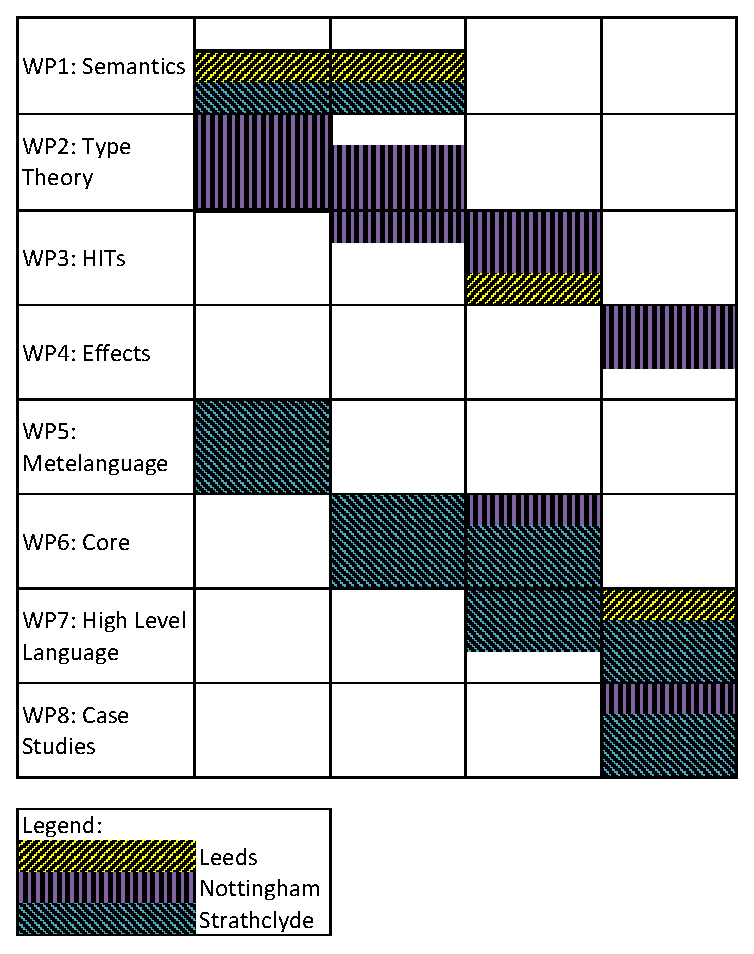
\includegraphics{Gantt.eps}
%\caption{Gantt chart depicting the order and division of work on workpackages}
%\end{figure}
%\newpage

\begin{footnotesize}
\begin{twocolumn}
\bibliographystyle{plain}
%\bibliographystyle{abbrv}
%\bibliographystyle{plainnat}
\bibliography{proposal,alti,nicola}
\end{twocolumn}
\end{footnotesize}

% \begin{multicols}{2}
% \bibliographystyle{plain}
% \bibliography{proposal,alti}
% \end{multicols}{2}

\end{document}
